\pdfoutput=1

\documentclass[runningheads]{llncs}

% ---------------------------------------------------------------
% Include basic ECCV package
 
% TODO REVIEW: Insert your submission number below by replacing '*****'
% TODO FINAL: Comment out the following line for the camera-ready version
% \usepackage[review,year=2024,ID=8270]{eccv}
% TODO FINAL: Un-comment the following line for the camera-ready version
% \usepackage{eccv}

% OPTIONAL: Un-comment the following line for a version which is easier to read
% on small portrait-orientation screens (e.g., mobile phones, or beside other windows)
\usepackage[mobile]{eccv}


% ---------------------------------------------------------------
% Other packages

% Commonly used abbreviations (\eg, \ie, \etc, \cf, \etal, etc.)
\usepackage{eccvabbrv}

% Include other packages here, before hyperref.
\usepackage{graphicx}
\usepackage{booktabs}

% The "axessiblity" package can be found at: https://ctan.org/pkg/axessibility?lang=en
\usepackage[accsupp]{axessibility}  % Improves PDF readability for those with disabilities.

% CUSTOM PACKAGES
\usepackage[table]{colortbl}
\usepackage{verbatim}
\usepackage{setspace}


% ---------------------------------------------------------------
% Hyperref package

% It is strongly recommended to use hyperref, especially for the review version.
% Please disable hyperref *only* if you encounter grave issues.
% hyperref with option pagebackref eases the reviewers' job, but should be disabled for the final version.
%
% If you comment hyperref and then uncomment it, you should delete
% main.aux before re-running LaTeX.
% (Or just hit 'q' on the first LaTeX run, let it finish, and you
%  should be clear).

% TODO FINAL: Comment out the following line for the camera-ready version
% \usepackage[pagebackref,breaklinks,colorlinks,citecolor=eccvblue]{hyperref}
% TODO FINAL: Un-comment the following line for the camera-ready version
\usepackage{hyperref}

% Support for ORCID icon
\usepackage{orcidlink}


\input{vincents_commands}
% Specific to the paper

\textvars{out,half}

\newcommand{\In}{\text{in}}
\newcommand{\Mid}{\text{mid}}

\newcommand{\innershift}{\delta^\In}
\newcommand{\outershift}{\delta^\out}
\newcommand{\propinnershift}{\epsilon^\In}
\newcommand{\propoutershift}{\epsilon^\out}


%SVG
% \usepackage{svg}
% \svgpath{{../images/}} % <- using \svgpath to avoid warning
\usepackage{adjustbox}

\addeditor{vincent}{VL}{0.0, 0.5, 0.0}
\addeditor{antoine}{AG}{0.0, 0.0, 0.8}
\showeditstrue
\showeditsfalse
\moretextwithfigures

\begin{document}

% ---------------------------------------------------------------
% TODO REVIEW: Replace with your title

\title{Gaussian Frosting: Editable Complex Radiance Fields with Real-Time Rendering}

% TODO REVIEW: If the paper title is too long for the running head, you can set
% an abbreviated paper title here. If not, comment out.
\titlerunning{Gaussian Frosting}

% TODO FINAL: Replace with your author list. 
% Include the authors' OCRID for the camera-ready version, if at all possible.
\author{
\vspace{-0.9cm} \> \\
Antoine Guédon\orcidlink{0009-0001-3107-4454} \and
Vincent Lepetit\orcidlink{0000-0001-9985-4433}
}

% TODO FINAL: Replace with an abbreviated list of authors.
\authorrunning{A.~Guédon and V.~Lepetit}
% First names are abbreviated in the running head.
% If there are more than two authors, 'et al.' is used.

% TODO FINAL: Replace with your institution list.
\institute{\vspace{-0.5cm} \> \\
\email{firstname.lastname@enpc.fr}\\
LIGM, Ecole des Ponts, Univ Gustave Eiffel, CNRS, France\\
{\tt\small \url{https://anttwo.github.io/frosting/}}
}

\maketitle

\begin{abstract}
\vspace{-1.5cm}
\begin{figure}[ht]
  \centering
  %
  \begin{subfigure}{0.31\linewidth}
  \includegraphics[width=\linewidth]{images/renders/bicycle_rgb_52.jpg}
  \end{subfigure}
  \hfill
  \begin{subfigure}{0.31\linewidth}
  \includegraphics[width=\linewidth]{images/renders/buzz1_rgb_49.jpg}
  \end{subfigure}
  \hfill
  \begin{subfigure}{0.31\linewidth}
  \includegraphics[width=\linewidth]{images/renders/kitten_rgb_42.jpg}
  \end{subfigure}\\
  {\small (a)~Rendering three different scenes with Frosting: \textit{Bicycle}, \textit{Buzz}, and \textit{Kitten}.}\\
  %
  \begin{subfigure}{0.49\linewidth}
  \includegraphics[width=\linewidth]{images/composition/buzz_riding_cat/0_0.png}
  \includegraphics[width=\linewidth]{images/composition/buzz_riding_cat/0_3.png}
  \end{subfigure}
  \hfill
  \begin{subfigure}{0.49\linewidth}
  \includegraphics[width=\linewidth]{images/composition/buzz_riding_cat/0_1.png}
  \includegraphics[width=\linewidth]{images/composition/buzz_riding_cat/0_2.png}
  \end{subfigure}
  {\small (b)~Composition: \textit{Buzz is riding a giant kitten jumping over a bench.}}\\
  %
  \begin{subfigure}{0.49\linewidth}
 \includegraphics[width=0.49\linewidth]{images/composition/buzz_riding_cat/closeup_1.png}
 \includegraphics[width=0.49\linewidth]{images/composition/buzz_riding_cat/closeup_2.png}
 \caption*{(c) Fuzzy details rendered with Frosting - occlusions are correctly rendered}
  \end{subfigure}
  %
  \hfill
  %
  \begin{subfigure}{0.49\linewidth}
  \includegraphics[width=0.49\linewidth]{images/composition/buzz_riding_cat/closeup_1_flat.png}
 \includegraphics[width=0.49\linewidth]{images/composition/buzz_riding_cat/closeup_2_flat.png}
  \caption*{(d) Rendering with SuGaR~\cite{guedon2023sugar} - the fur does not occlude the legs correctly}
  \end{subfigure}
  %
  \caption{
  % original caption
  % \textbf{Complex scene composition with Frosting.} Frosting has editing capabilities similar to surface-based methods like SuGaR~\cite{guedon2023sugar}, but reaches better performance for rendering complex volumetric effects such as fuzzy materials. In this example, we were able to animate both Buzz and the kitten, changing their original pose (a) while preserving high-quality rendering (b): Contrary to SuGaR, very fine and fuzzy details such as the kitten's hair can be seen covering Buzz's legs in a realistic way (c).
  % final caption
  We propose to represent surfaces by a mesh covered with a ``Frosting'' layer of varying thickness and made of 3D Gaussians. This representation captures both complex volumetric effects created by fuzzy materials such as the cat's hair or grass as well as flat surfaces. 
  Built from RGB images only, it can be rendered in real-time and animated using traditional animation tools.
  In the example above, we were able to animate both Buzz and the kitten, changing their original pose (a) while preserving high-quality rendering (b): Contrary to SuGaR, very fine and fuzzy details such as the kitten's hair can be seen covering Buzz's legs in a realistic way (c).
  }
  \label{fig:sugar-comparison}
\end{figure}
\begin{figure}[h]
  \centering
  
  
   \begin{subfigure}{0.49\linewidth}
  \includegraphics[width=0.99\linewidth]{images/renders/panda1_rgb_166.jpg}
  \caption{Rendering}
  \end{subfigure}
  \hfill
  \begin{subfigure}{0.49\linewidth}
  \includegraphics[width=0.99\linewidth]{images/frosting_size/panda1_size_166.jpg}
  \caption{Thickness of the Frosting layer}
  \end{subfigure}
  
  % \includegraphics[height=6.5cm]{eijkel2}
  % \fbox{\rule{0pt}{2in} \rule{.9\linewidth}{0pt}}
  \caption{
  % We propose to represent surfaces by a mesh covered with a ``frosting'' layer of varying thickness and made of 3D Gaussians. This representation captures both complex volumetric effects created by fuzzy materials such as the cat's hair as well as flat surfaces. It can be rendered in real-time and animated using traditional animation tools as shown in the video provided as supplementary material. We also propose a method to build this representation from color images and capture fine details as seen in the rendered image and the normal map.
  \textbf{Visualization of the thickness of the Frosting layer on an example.} A thicker layer is shown with a brighter value. Our method automatically builds a thick Frosting layer for fuzzy areas  such as the fur of the red panda plush, and a thin Frosting layer for flat surfaces such as the table or the floor. Adapting the thickness of the Frosting layer allows for allocating more Gaussians in areas where more volumetric rendering is necessary near the surface, resulting in an efficient distribution of Gaussians in the scene. As we demonstrate in the paper, using an adaptive thickness results in higher performance than using a predefined constant thickness, and reduces artifacts when animating the mesh.}
  \label{fig:teaser}
\end{figure}
\input{0b_abstract}
\end{abstract}

\vspace{1cm}
\vspace{-10pt}
\section{Introduction}
\label{sec:intro}
Autoregressive (AR) and diffusion models are two powerful paradigms for data distribution modeling. AR models, also known as the next token prediction approach, dominate language modeling and are considered central to the success of large language models (LLMs)~\cite{gpt1,gpt2,gpt3,llama1,llama2,llama3}. On the other hand, diffusion models~\cite{ddpm,dit,adm,edm}, or score-based generative models~\cite{songscore,lipman2023flow}, have emerged as the leading approach for visual generation, driving unprecedented progress in the era of visual content generation~\cite{sora,rombach2022high,li2023scaling}. 

\begin{figure}[t]
    \centering
    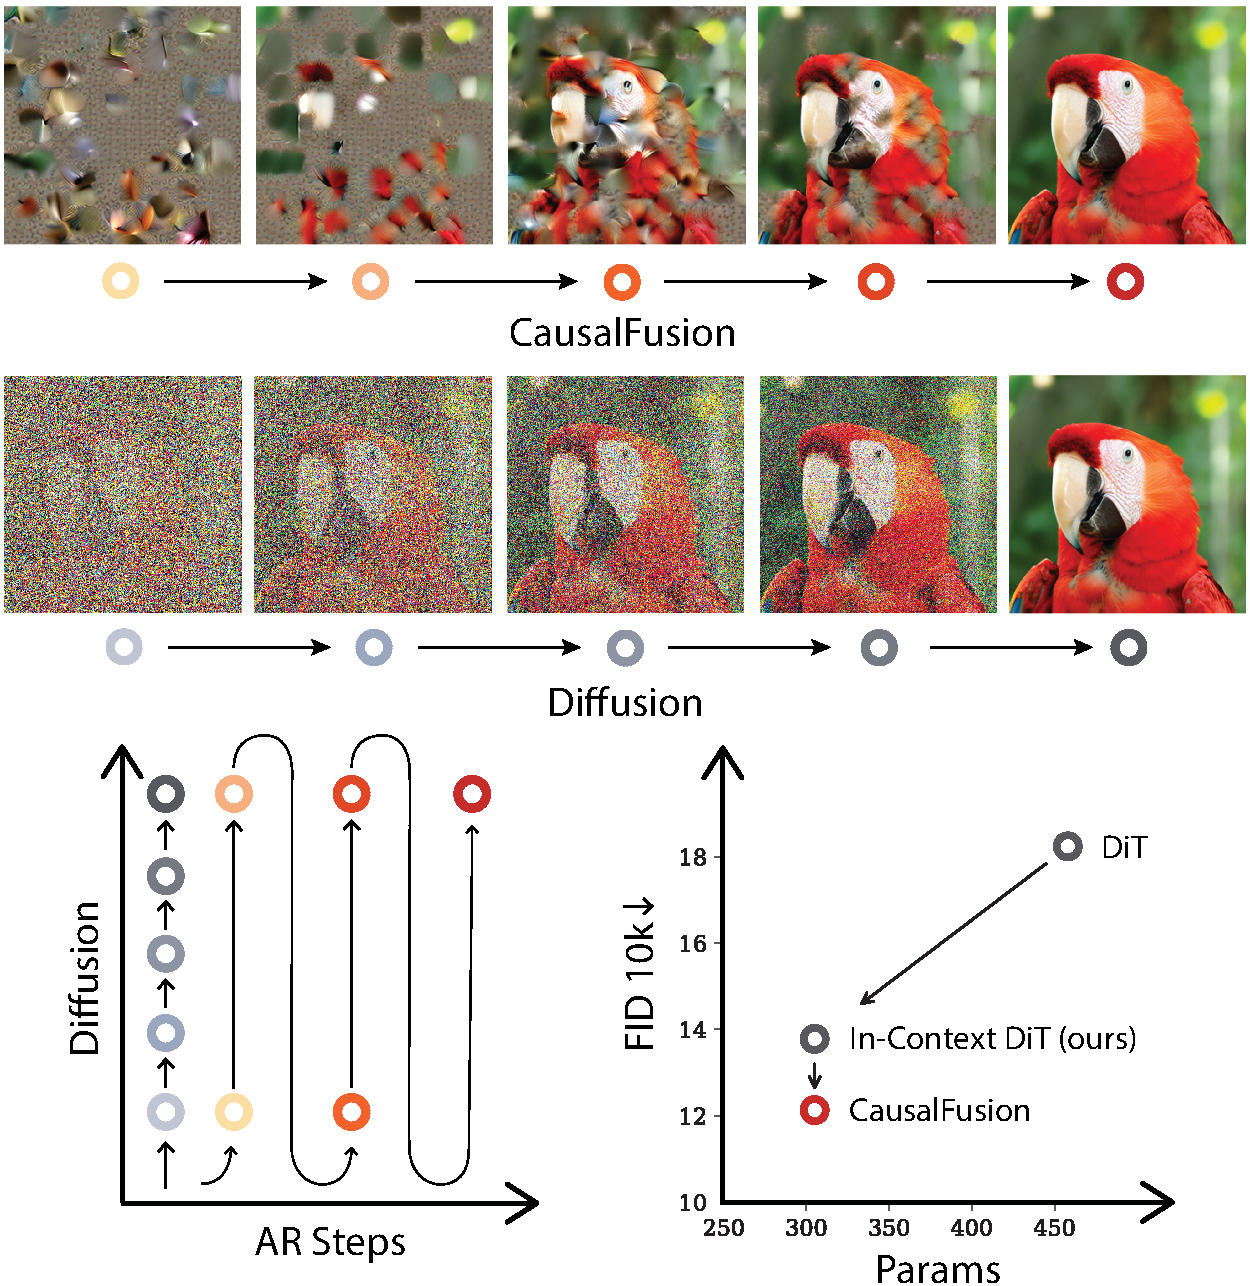
\includegraphics[width=1.0\textwidth,height=1.0\textwidth]{figs/casualfusion-teaser-v6.pdf} 
    \vspace*{-6mm}
    \caption{
    \textbf{Illustration of Dual-Factorization}. The arrow line indicates CausalFusion's generation path, moving from one state to the next by jointly generating along the sequential and noise-level dimension at each step. 
    Compared to DiT, our In-context DiT substantially improves results with fewer parameters. CausalFusion further enhances performance without changing the architecture or parameter count. Results were trained on IN1K for 240 epochs. CausalFusion adopts arbitrary AR steps for image generation, but each step only diffuses partial tokens, resulting in similar (or slightly lower) computational complexity.
    \vspace{-10pt}
    }
    \label{fig:dual-factorization}
\end{figure}


\begin{figure*}[t]
  \centering
  \begin{subfigure}{1.0\linewidth}
    \centering
    \includegraphics[width=\linewidth]{figs/figure2.pdf}
    \caption{Samples generated by CausalFusion-XL/2, ImageNet 512$\times$512, 800 epoch, DDPM 250 steps, CFG=4.0}
  \end{subfigure}
  \begin{subfigure}{1.0\linewidth}
    \centering
    \includegraphics[width=\linewidth]{figs/edit.pdf}
    \caption{\textbf{Zero-shot image editing} results generated by CausalFusion-XL/2, ImageNet 512$\times$512, 800 epoch. We first generate the original image (those on the left), then mask out its centre region, top-half, or bottom-half, and regenerate the image with new class conditions. Details are discussed in Sec \ref{sec:system}.}
  \end{subfigure}
  \caption{\textbf{Visualization results}. All samples are generated by models trained only on \textbf{ImageNet-1K class-conditional generation} task, demonstrating CausalFusion's zero-shot image manipulation ability. See more visualization results in Appendix~\ref{appendix:secD}.
  \vspace{-12pt}
  }
  \vspace{-6pt}
  \label{fig:vis1}
\end{figure*}

The intrinsic distinction between AR and diffusion models lies in their approach to data distribution factorization. AR models treat data as an ordered sequence, factorizing it along the sequential axis, where the probability of each token is conditioned on all preceding tokens. This factorization enables the AR paradigm to generalize effectively and efficiently across arbitrary number of tokens, making it well-suited for long-sequence reasoning and in-context generation. In contrast, diffusion models factorize data along the noise-level axis, where the tokens at each step are a refined (denoised) version of themselves from the previous step. As a result, the diffusion paradigm is generalizable to arbitrary number of data refinement steps, enabling iterative quality improvement with scaled inference compute. While AR and diffusion models each excel within their respective domains, their distinct factorization approaches reveal complementary potential. Although recent studies~\cite{transfusion,monoformer,dart} have attempted to integrate AR and diffusion within a single model, they typically treat these paradigms as separate modes, missing the potential benefits of jointly exploring them within a 2-D factorization plane.

To this end, we introduce \textbf{CausalFusion}, a flexible framework that integrates both sequential and noise-level data factorization to unify their advantages. The degree of factorization along these two axes—namely, the AR step and diffusion step—is adjustable, enabling {CausalFusion} to revert seamlessly to the traditional AR or diffusion paradigms at either extreme. To enhance its generality, CausalFusion is designed to predict \textit{any} number of tokens at \textit{any} AR step, with \textit{any} pre-defined sequence order and \textit{any} level of inference compute, thereby minimizing the inductive biases presented in existing generative models. As shown in Figure~\ref{fig:dual-factorization}, this approach provides a broad spectrum between the AR and diffusion paradigms, allowing smooth interpolation within two endpoints during both training and inference. 
Specifically, we explore CausalFusion in image generation and multimodal generation scenarios, where we observe that the level of training difficulties significantly influences the overall effectiveness of CausalFusion.

\textbf{Difficulties of generative tasks in CausalFusion:} Both AR and diffusion paradigms present unique challenges based on difficulties of their specific generative stages. In diffusion models, the effectiveness of training depends heavily on proper loss weighting across noise levels~\cite{ddpm,minsnr}, as higher noise levels are more difficult and usually provide more valuable signals than lower noise levels. Similarly, AR models are susceptible to error accumulation~\cite{bengio2015scheduled} as early-stage predictions are made with limited visible context, making them more error-prone. Optimizing CausalFusion thus requires balancing across these varying task difficulties to optimize training signal impact and ensure sufficient exploration across the entire factorization plane.

In this paper, we formally examine the difficulties of generative tasks within CausalFusion. We show that, in addition to the noise levels in diffusion and the amount of visible context in AR, the total number of AR steps, which controls the interpolation between AR and diffusion, also plays a critical role in shaping training difficulties. Driven by these factors, we develop a scalable and versatile model based on the CausalFusion framework. Starting from the DiT architecture~\cite{dit}, we gradually convert it into a decoder-only transformer compatible with existing AR models like GPT~\cite{gpt1,gpt2,gpt3} and LLaMA~\cite{llama1,llama2,llama3}. We provide insights on how to appropriately choose the number of AR steps during the training of CausalFusion models, and further introduce loss weighing along both the diffusion and AR axis to balance the impact of different generative stages. As shown in Figure~\ref{fig:dual-factorization} and ~\ref{fig:vis1}, our model achieves state-of-the-art performance on the ImageNet class-conditional generation benchmark, significantly outperforming DiT~\cite{dit} and enabling zero-shot image manipulations due to its AR nature. When pretraining on both text-to-image and image-to-text tasks, our model surpasses forced-fusion frameworks such as TransFusion~\cite{transfusion}, demonstrating the versatility of our CausalFusion framework.


We highlight our main contribution below:
\begin{itemize}
\item  We propose CausalFusion as the AR counterpart to DiT, achieving state-of-the-art results and enabling the unlimited token generation for in-context reasoning.
\item  We systematically study CausalFusion on the dual-factorization plane and identify key factors that improve the effectiveness of CausalFusion models.
\item  Compared with recent studies~\cite{transfusion}, CausalFusion enables a smooth, cohesive integration with language modeling for cross-modal generation and reasoning.
\end{itemize} 

\section{Related Work}
\label{sec:related work}

\begin{figure*}[t]
    \centering
    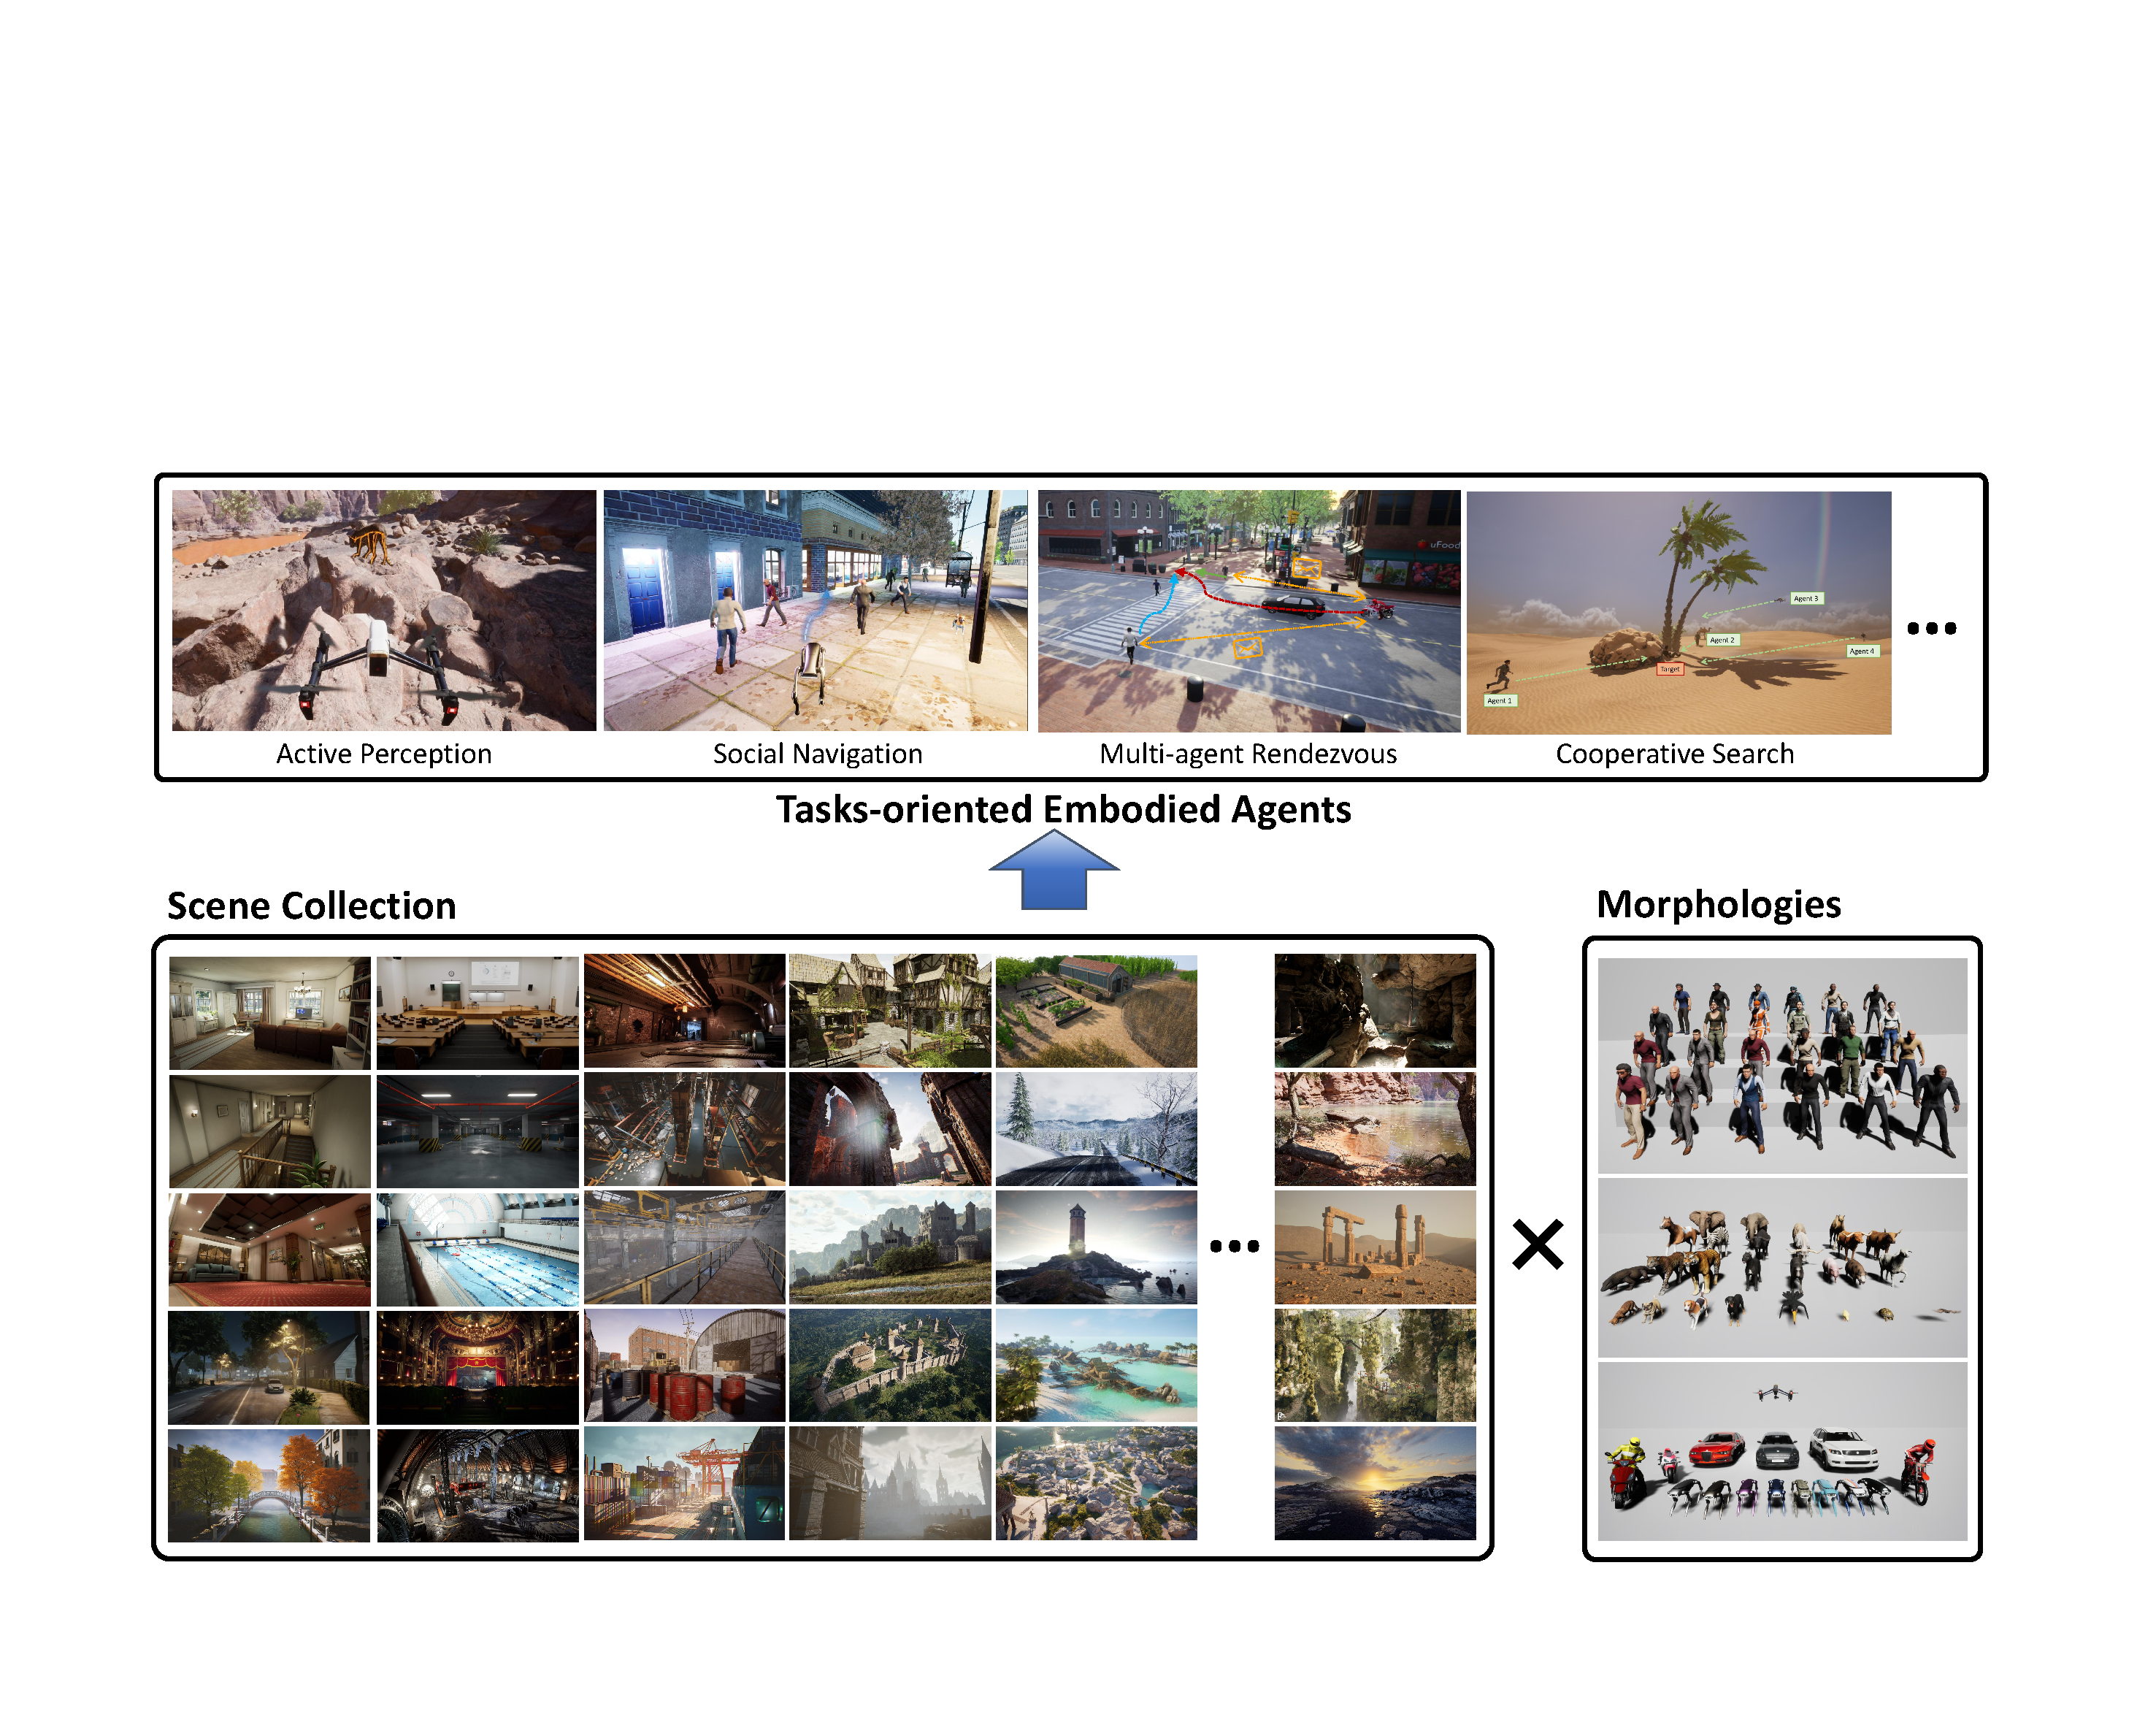
\includegraphics[width=1\linewidth]{figure/overview.pdf}\vspace{-2mm}
    \caption{Overview of the proposed~\name.}
    \label{fig:overview}
\end{figure*}

% \textbf{Video Super-Resolution.}
\paragraph{Video Super-Resolution.} 
Traditional VSR methods can be roughly divided into two categories: recurrent-based \cite{haris2019recurrent, huang2017video, liang2022recurrent, sajjadi2018frame, shi2022rethinking} and sliding-window-based \cite{caballero2017real,liang2024vrt,li2020mucan,xu2021temporal,yi2019progressive} methods. 
Recurrent-based methods process LR video frame by frame using recurrent neural networks \cite{mikolov2010recurrent}. In contrast, sliding-window-based methods divide a video sequence into segments, using each as input to super-resolve the video. 
However, both approaches suffer from degradation mismatch, leading to significant performance drops in real-world applications.
Recently, there has been a growing focus on real-world VSR, targeting complex, unknown degradations. RealBasicVSR \cite{chan2022investigating}, an extension of BasicVSR \cite{chan2021basicvsr}, introduces a pre-cleaning module to mitigate artifacts. 
RealViformer \cite{zhang2024realviformer} discovers that channel attention is less sensitive to artifacts and uses squeeze-excite mechanisms and covariance-based rescaling to address these challenges further. While GAN-based and image diffusion models have made substantial progress, they still face issues such as \textit{over-smoothing details and temporal inconsistency}.

\vspace{-1em}
\paragraph{Text-to-Video Diffusion Model.} 
% \noindent
% \textbf{Text-to-Video Diffusion Model.}
Large-scale pre-trained text-to-video (T2V) diffusion models have garnered significant attention, particularly with the impressive results from Sora \cite{videoworldsimulators2024,sora}. 
Numerous T2V models have since emerged, generally divided into: U-Net-based methods \cite{blattmann2023align, blattmann2023stable, ho2022imagen, singer2022make} and DiT-based methods \cite{yang2024cogvideox, bao2024vidu, polyak2024movie, chen2024gentron}. 
I2VGen-XL \cite{zhang2023i2vgen}, a U-Net-based method, employs a two-stage approach: first generating semantically and content-consistent LR videos, then using these as conditions to produce HR outputs.
CogvideoX \cite{yang2024cogvideox}, built on DiT \cite{peebles2023scalable}, introduces an adaptive LayerNorm to enhance text-video alignment and employs 3D attention to better integrate spatio-temporal information.
Both models %, regardless of architecture, 
have large model capacities and are trained on large-scale datasets, enabling them to capture robust spatio-temporal priors. 
In this work, we propose~\name~to \textit{fully leverage T2V model prior for real-world VSR}.

\vspace{-1em}
\paragraph{Diffusion Prior for Super-Resolution.}
% \noindent
% \textbf{Diffusion Prior for Super-Resolution.}
Several works \cite{wang2024exploiting, lin2023diffbir, yang2023pixel, wu2024seesr, zhao2024wavelet} have leveraged generative diffusion priors for image and video super-resolution. 
StableSR \cite{wang2024exploiting} adds a time-aware encoder and feature warping module to the SD model. DiffBIR \cite{lin2023diffbir} integrates restoration and generative modules via ControlNet, while PASD \cite{yang2023pixel} and SeeSR \cite{wu2024seesr} embed semantic information in U-Net to guide diffusion. These methods balance fidelity and perceptual quality, achieving high-resolution image details.
Methods like Upscale-A-Video \cite{zhou2024upscale}, MGLD-VSR \cite{yang2023mgldvsr}, Inflating with Diffusion \cite{yuan2024inflation}, and SATeCo \cite{chen2024learning} have adapted text-to-image diffusion priors~\cite{rombach2022high,ho2022imagen} for VSR by adding temporal layers. However, rooted in text-to-image models, they often struggle with temporal consistency. 
More recently, VEnhancer\cite{he2024venhancer} and LaVie-SR\cite{wang2023lavie} have incorporated T2V models to super-resolve AI-generated videos but struggle with complex degradations in practical environments. 
In contrast, we are the \textit{first} to integrate powerful T2V diffusion priors for real-world VSR, introducing the LIEM module to address spatial artifacts and DF loss to enhance fidelity.
\section{3D Gaussian Splatting and Surface Reconstruction}

Our method relies on the original 3D Gaussian Splatting~(3DGS) method~\cite{kerbl3Dgaussians} for initialization and on SuGaR~\cite{guedon2023sugar} to align Gaussians with the surface of the scene and facilitate the extraction of a mesh. We briefly describe 3DGS and SuGaR in this section before describing our method in the next section.


\subsection{3D Gaussian Splatting} 

3DGS represents the scene as a large set of Gaussians. Each Gaussian $g$ is equipped with a mean $\mu_g\in \IR^3$ and a positive-definite covariance matrix $\Sigma_g\in \IR^{3\times 3}$. The covariance matrix is parameterized by a scaling vector $s_g\in\IR^3$ and a quaternion $q_g\in\IR^4$ encoding the rotation of the Gaussian. 

In addition, each Gaussian has a view-dependent radiance represented by an opacity $\alpha_g\in [0,1]$ and a set of spherical harmonics coordinates defining the colors emitted for all directions. To render an image from a given viewpoint, a rasterizer ``splats'' the 3D Gaussians into 2D Gaussians parallel to the image plane and blends the splats depending on their opacity and depth. This rendering is extremely fast, which is one of the advantages of 3DGS over volumetric rendering as in NeRFs for example~\cite{mildenhall2020nerf, mueller2022instantngp, barron2022mipnerf360}.


Gaussian Splatting can be seen as an approximation of the traditional volumetric rendering of radiance fields with the following density function $d$, computed as the sum of the Gaussian values weighted by their alpha-blending coefficients at any 3D point $p\in \IR^3$:
%
 \begin{equation}
    d(p) = \sum_{g} \alpha_g \exp\left(-\frac{1}{2}(p - \mu_g)^T \Sigma^{-1}_g (p - \mu_g)\right) \> .
    \label{eq:gaussian_splatting_density}
\end{equation}

We initialize our Gaussian Frosting method using a vanilla 3DGS optimization: Gaussians are initialized using the point cloud produced by an SfM~\cite{snavely-2006-structure-from-motion} algorithm like COLMAP~\cite{schoenberger2016mvs,schoenberger2016sfm}, required to compute camera poses. The Gaussians' parameters (3D means, scaling vectors, quaternions, opacities, and spherical harmonics coordinates) are then optimized to make the renderings match the ground truth images of the scene, using a rendering loss that only consists in a combination of a pixel-wise L1 distance and a more structural D-SSIM term. 


\subsection{SuGaR Mesh Extraction} 

Vanilla 3DGS does not have regularization explicitly encouraging Gaussians to align with the true surface of the scene. Our Gaussian Frosting representation relies on a mesh that approximates this surface, in order to be editable by traditional tools. To obtain this mesh, we rely on the method proposed in SuGaR~\cite{guedon2023sugar}, which we improve by automatically selecting a critical hyperparameter.

SuGaR proposes a regularization term encouraging the alignment of the 3D Gaussians with the true surface of the scene during the optimization of Gaussian Splatting, as well as a mesh extraction method. After enforcing the regularization, the optimization provides Gaussians that are mostly aligned with the surface albeit not perfectly: We noticed that in practice, a large discrepancy between the regularized Gaussians and the extracted mesh indicates the presence of fuzzy materials or surfaces that require volumetric rendering. We thus exploit this discrepancy as a cue to evaluate where the Frosting should be thicker.

\begin{figure}[tb]
  \centering
  % \includegraphics[height=6.5cm]{eijkel2}
  % \fbox{\rule{0pt}{0.8in} \rule{.95\linewidth}{0pt}}
  %\includesvg[inkscapelatex=false, width = 1\linewidth]{images/pipeline_frosting_largefont}
  \includegraphics[width=\linewidth]{images/pipeline_frosting_largefont.pdf}
  \caption{
  \textbf{Creating a Layer of Gaussian Frosting.} To build our proposed Frosting representation, we start by optimizing a Gaussian Splatting representation using a rendering loss without any additional constraint, to let Gaussians position themselves. We refer to these Gaussians as \emph{unconstrained}. We then regularize these Gaussians to enforce their alignement with the surface, and extract a mesh that will serve as a basis for the Frosting. Next, we use the misalignment of surface-aligned Gaussians to identify areas where more volumetric rendering is needed, and we build search intervals $J_i$ around the mesh's vertices $\vec{v_i}$. Finally, we use the density function of the unconstrained Gaussians to refine the intervals, resulting in a Frosting layer. We finally sample a novel, densified set of Gaussians inside the layer.
}
  \label{fig:frosting-pipeline}
\end{figure}

\section{Creating a Frosting Layer from Images}

In this section, we describe our Gaussian Frosting creation method: 
First, we extract an editable surface with optimal resolution using SuGaR. We then detail how we use this surface-based model to go back to a volumetric but editable representation built around the mesh. This representation adapts to the complexity of the scene and its need for more volumetric effects. Finally, we describe how we parameterize and refine this representation. An overview is provided Figure~\ref{fig:frosting-pipeline}.

\subsection{Forward Process: From Volume to Surface}
\label{subsec:forward-process}

We start by optimizing an unconstrained Gaussian Splatting representation for a short period of time to let Gaussians position themselves. We will refer to such Gaussians as \emph{unconstrained}. We save these Gaussians aside, and apply the regularization term from SuGaR to enforce the alignment of the Gaussians with the real surface. We will refer to these Gaussians as \emph{regularized}.

Once we obtain the regularized Gaussians, we extract a surface mesh from the Gaussian Splatting representation. This surface mesh serves as a basis for our representation. Like SuGaR~\cite{guedon2023sugar}, we then sample points on the visible level set of the Gaussian splatting density function, and apply Poisson reconstruction. 

In the supplementary material, we describe our technique to automatically estimate a good value for a critical hyperparameter used by Poisson reconstruction, namely the octree depth $D$. As we will show in the Experiments section, selecting the right value for $D$ when applying Poisson reconstruction can drastically improve both the quality of the mesh and the rendering performance of our model. Figure~\ref{fig:mesh-comparison} illustrates this point.


\begin{figure}[tb]
  \centering
  \begin{subfigure}{0.19\linewidth}
  \includegraphics[width=\linewidth]{images/meshes/khady_sugar.png}
  \end{subfigure}
  %
  \hfill
  %
  \begin{subfigure}{0.19\linewidth}
  \includegraphics[width=\linewidth]{images/meshes/pug_sugar.png}
  \end{subfigure}
  %
  \hfill
  %
  \begin{subfigure}{0.19\linewidth}
  \includegraphics[width=\linewidth]{images/meshes/horse_y_sugar.png}
  \end{subfigure}
  %
  \hfill
  %
  \begin{subfigure}{0.19\linewidth}
  \includegraphics[width=\linewidth]{images/meshes/kitten_sugar.png}
  \end{subfigure}
  %\hfill
  %
  % \begin{subfigure}{0.19\linewidth}
  % \includegraphics[width=\linewidth]{images/meshes/woolly_sugar.png}
  % \end{subfigure}
  %
  %
  \vspace{0.005\linewidth}\\
  {\small (a) Using the predefined, large parameter $D$ as in SuGaR~\cite{guedon2023sugar}} 
  % \vspace{0.01\linewidth}
  \\
  %
  \begin{subfigure}{0.19\linewidth}
  \includegraphics[width=\linewidth]{images/meshes/khady_frosting.png}
  \end{subfigure}
  %
  \hfill
  %
  \begin{subfigure}{0.19\linewidth}
  \includegraphics[width=\linewidth]{images/meshes/pug_frosting.png}
  \end{subfigure}
  %
  \hfill
  %
  \begin{subfigure}{0.19\linewidth}
  \includegraphics[width=\linewidth]{images/meshes/horse_y_frosting.png}
  \end{subfigure}
  %
  \hfill
  %
  \begin{subfigure}{0.19\linewidth}
  \includegraphics[width=\linewidth]{images/meshes/kitten_frosting.png}
  \end{subfigure}
  %
  % \hfill
  % %
  % \begin{subfigure}{0.19\linewidth}
  % \includegraphics[width=\linewidth]{images/meshes/woolly_frosting.png}
  % \end{subfigure}
  %
  % \vspace{0.005\linewidth}
  \\
  {\small (b) Using our automatically computed $D$ that adapts to the complexity of the 3DGS}
  %
  \caption{
  \textbf{Comparison of meshes extracted by SuGaR from the Shelly dataset without and with our improvement that automatically tunes the octree depth $D$ in Poisson reconstruction depending on the complexity of the scene.}
  Our technique~(bottom) drastically reduces surface artifacts for many scenes, such as the holes and the ellipsoidal bumps on the surface when using the default values from~\cite{guedon2023sugar}~(top).
}
  % \vincentrmk{I would remove the purple thing on the right, the 2 meshes are not very different}
%  \vincentrmk{I removed the wooly thing}
  % Moreover, the outer bound of the frosting layer~(bottom), which is computed using the unconstrained, non-aligned Gaussians, generally provides a refined mesh with better quality than the mesh directly obtained from the isosurface of the aligned Gaussians.
  
  
    % \textbf{Comparison of meshes reconstructed from Gaussian Splatting representations using SuGaR~\cite{guedon2023sugar} and our approach.}
  % Our method to compute automatically optimal hyperparameters for Poisson recontruction~(center) drastically reduces surface artifacts for a lot of scenes, such as the ellipsoidal bumps on the surface when using the default values from~\cite{guedon2023sugar}~(left). Moreover, the outer bound of the frosting layer~(right), which is computed using the unconstrained, non-aligned Gaussians, generally provides a refined mesh with better quality than the mesh directly obtained from the isosurface of the aligned Gaussians.}}
  \label{fig:mesh-comparison}
\end{figure}
% \todo{We also follow SuGaR~\cite{guedon2023sugar} for extracting a base mesh, but we can actually give more details as shown above. Indeed, SuGaR is very elusive on this part; I think it's interesting to understand what Poisson reconstruction provides, that the density functions lacks. Moreover, this part may be important to explain the improvement that I a added, which is a way to automatically compute the optimal octree depth hyperparameter for Poisson reconstruction depending on the configuration of the Gaussians in the scene. This greatly helps to remove "blobs" in the scene without having to tweak the octree depth parameter by hand, so it could be a contribution. Having a well-balanced mesh is important to get a nice frosting.}


\subsection{Backward Process: From Surface to Volume}
\label{sec:shifts}

After extracting a base mesh, we build a Frosting layer with a variable thickness and containing Gaussians around this mesh. We want this layer to be thicker in areas where more volumetric rendering is necessary near the surface, such as fuzzy material like hair or grass for example. On the contrary, this layer should be very thin near the parts of the scene that corresponds to well-defined flat surfaces, such as wood or plastic for example.

\begin{figure}[t]
  \centering
  % \includesvg[inkscapelatex=false, width = 1\linewidth]{images/ray.svg}
  % \includesvg[inkscapelatex=false, width = 1\linewidth]{images/ray.svg}
  % \includesvg[inkscapelatex=false, width = 1\linewidth]{images/ray_w_mesh.svg}
  \includegraphics[width=\linewidth]{images/ray_w_mesh.pdf}
  \caption{
  \textbf{How we define the inner and outer bounds of the Frosting layer.} See text in Section~\ref{sec:shifts}.}
  \label{fig:shifts}
\end{figure}


As illustrated in Figure~\ref{fig:shifts}, to define this layer, we introduce two values $\innershift_i$ and $\outershift_i$ for each vertex $\vec{v}_i$ of the extracted base mesh $\calM$. This gives two surfaces with vertices $(\vec{v}_i+\innershift_i \vec{n}_i)_i$ and $(\vec{v}_i+\outershift_i \vec{n}_i)_i$ respectively, where $\vec{n}_i$ is the mesh normal at vertex $\vec{v}_i$. These two surfaces define the inner and outer bounds of the Frosting layer. Note that we do not have to build them explicitly as they directly depend on the base mesh and the $\innershift_i$'s and $\outershift_i$'s.


To find good values for the $\innershift_i$'s and $\outershift_i$'s, we initially tried using directly the unconstrained Gaussians, i.e., the Gaussians obtained before applying the regularization term from SuGaR.  Unfortunately, without regularization, Gaussian Splatting tends to retrieve a thick layer of Gaussians even for ``non-fuzzy'' surfaces, which would result in excessively large values for $\innershift_i$ and $\outershift_i$.  Moreover, the unconstrained Gaussians generally contain many transparent floaters and other outlier Gaussians. Such Gaussians could also bias the shifts toward unnecessarily large values. On the other hand, using only the regularized Gaussians to setup the $\innershift_i$'s and $\outershift_i$'s could miss fuzzy areas since these Gaussians are made flatter by the regularization.


Our solution is thus to consider both the unconstrained and the regularized Gaussians.  More exactly, we estimate the Frosting thickness from the thickness of the unconstrained Gaussians by looking for their isosurfaces, BUT, to make sure we consider the isosurfaces close to the scene surface, we search for the isosurfaces close to the regularized Gaussians: Even under the influence of the regularization term from SuGaR, Gaussians do not align well with the geometry around surfaces with fuzzy details.  As a consequence, the local thickness of the regularized Gaussians is a cue on how fuzzy the material is.


Figure~\ref{fig:shifts}  illustrates what we do to fix the $\innershift_i$'s and $\outershift_i$'s. To restrict the search, we define a first interval $I_i = [-3\sigma_i, 3\sigma_i]$ for each vertex $\vec{v}_i$, where $\sigma_i$ is the standard deviation in the direction of $\vec{n}_i$ of the regularized Gaussian the closest to $\vec{v}_i$. $I_i$ is the confidence interval for the 99.7 confidence level of the 1D Gaussian function of $t$ along the normal. Fuzzy parts result in general in large $I_i$. We could use the $I_i$'s to restrict the search for the isosurfaces of the unconstrained Gaussians. A more reliable search interval $J_i$ is obtained by looking for the isosurfaces of the regularized Gaussians along  $\vec{n}_i$ within $I_i$:
%
\begin{equation}
    \propinnershift_i = \inf ( T ) \text{ , }
    \propoutershift_i = \sup ( T ) \text{ , with }
    T = \left\{ t\in I_i \>\> | \>\> d_r(\vec{v}_i+t\vec{n}_i) \geq \lambda \right\} \> ,
    \label{eq:proposal-shifts}
\end{equation}
%
where $d_r$ is the density function as defined in Eq.~\eqref{eq:gaussian_splatting_density} for the regularized Gaussians.  In practice, we use an isosurface level~$\lambda = 0.01$, i.e., close to zero.
%
We use $ \propinnershift_i$ and $\propoutershift_i$ to define interval $J_i$: $J_i = \left[ \epsilon^\Mid_i - k\epsilon^\half_i, \epsilon^\Mid_i + k\epsilon^\half_i \right]$, with $\epsilon^\Mid_i = (\propinnershift + \propoutershift)/2$ and $\epsilon^\half_i = (\propoutershift - \propinnershift)/2$. We take $k=3$ as it gives an interval large enough to include most of the unconstrained Gaussians while rejecting the outlier Gaussians. Finally, we can compute the inner and outer shifts~$\innershift_i$ and $\outershift_i$ as:
%
\begin{equation}
    \innershift_i = \inf ( V ) \text{ , }
    \outershift_i = \sup ( V ) \text{ , with }
    V = \left\{ t\in J_i \>\> | \>\> d_u(\vec{v}_i+t\vec{n}_i) \geq \lambda \right\} \> .
    \label{eq:shifts}
\end{equation}

\begin{figure}[tb]
  \centering
  \begin{subfigure}{0.155\linewidth}
  \includegraphics[width=\linewidth]{images/renders/khady_rgb_31.jpg}
  \includegraphics[width=\linewidth]{images/normals/khady_normals_31.jpg}
  \includegraphics[width=\linewidth]{images/frosting_size/khady_size_31.jpg}
  \end{subfigure}
  %
  \hfill
  %
  \begin{subfigure}{0.155\linewidth}
  \includegraphics[width=\linewidth]{images/renders/faraam0_rgb_14.jpg}
  \includegraphics[width=\linewidth]{images/normals/faraam0_normals_14.jpg}
  \includegraphics[width=\linewidth]{images/frosting_size/faraam0_size_14.jpg}
  \end{subfigure}
  %
  \hfill
  %
  \begin{subfigure}{0.155\linewidth}
  \includegraphics[width=\linewidth]{images/renders/sirius1_rgb_52bis.jpg}
  \includegraphics[width=\linewidth]{images/normals/sirius1_normals_52_bis.jpg}
  \includegraphics[width=\linewidth]{images/frosting_size/sirius1_size_52_ter.jpg}
  \end{subfigure}
  %
  \hfill
  %
  \begin{subfigure}{0.155\linewidth}
  \includegraphics[width=\linewidth]{images/renders/garden_rgb_31.jpg}
  \includegraphics[width=\linewidth]{images/normals/garden_normals_31bis.jpg}
  \includegraphics[width=\linewidth]{images/frosting_size/garden_size_31bis.jpg}
  \end{subfigure}
  %
  \hfill
  %
  \begin{subfigure}{0.155\linewidth}
  \includegraphics[width=\linewidth]{images/renders/bicycle_rgb_52.jpg}
  \includegraphics[width=\linewidth]{images/normals/bicycle_normals_52bis.jpg}
  \includegraphics[width=\linewidth]{images/frosting_size/bicycle_size_52bis.jpg}
  \end{subfigure}
  %
  \caption{
  \textbf{Rendering complex scenes with Frosting.} First row: Renderings, Second row: recovered normal maps, Third row: estimated Frosting thickness. Note that the Frosting is thick on fuzzy materials such as the hair and the grass, as expected, and very thin on flat surfaces such as the table on the fourth column.
  }
  \label{fig:frosting-renders}
\end{figure}


\subsection{Frosting Optimization}

Once we constructed the outer and inner bounds of the Frosting layer, we initialize a densified set of Gaussians inside this layer and optimize them using 3DGS rendering loss as the unconstrained Gaussians. To make sure the Gaussians stay inside the frosting layer during optimization, we introduce a new parameterization of the Gaussians. Moreover, this parameterization will make possible to 
easily adjust the Gaussians' parameters when editing the scene.


\subsubsection{Parameterization.} Let us consider a triangular face of the base mesh $\calM$, with vertices denoted by~$\vec{v}_0, \vec{v}_1$, and~$\vec{v}_2$ and their corresponding normals~$\vec{n}_0, \vec{n}_1$, and~$\vec{n}_2$. After extracting inner and outer shifts from unconstrained Gaussians, we obtain six new vertices $(\vec{v}_i+\innershift_i \vec{n}_i)_{i=0,1,2}$ and $(\vec{v}_i+\outershift_i \vec{n}_i)_{i=0,1,2}$ that respectively belong to the inner and outer bounds of the frosting.
%
Specifically, these six vertices delimit an irregular triangular prism. We will refer to such polyhedrons as ``prismatic cells''. 
%
We parameterize the 3D mean~$\mu_g\in \IR^3$ of a Gaussian~$g \in \calG$ located inside a prismatic cell with a set of six barycentric coordinates split into two subsets~$(b_g^{(i)})_{i=0,1,2}$ and $(\beta_g^{(i)})_{i=0,1,2}$, such that 
%
\begin{equation}
    \mu_g = \sum_{i=0}^2 \left(
    b_g^{(i)} \left(\vec{v}_i+\outershift_i \vec{n}_i\right) +
    \beta_g^{(i)} \left(\vec{v}_i+\innershift_i \vec{n}_i\right)\right) \> ,
    \label{eq:barycentric-coordinates}
\end{equation}
%
with barycentric coordinates verifying $\sum_{i=0}^2 ( b_g^{(i)}+\beta_g^{(i)}) = 1$.
%
Using barycentric coordinates enforces Gaussians to stay inside their corresponding prismatic cell, and guarantees the stability of our representation during optimization.
%
In practice, we apply a softmax activation on the parameters to optimize to obtain barycentric coordinates that sum up to 1. 

\subsubsection{Initialization.} For a given budget $N$ of Gaussians provided by the user, we initialize $N$ Gaussians in the scene by sampling $N$ 3D centers $\mu_g$ in the frosting layer. Specifically, for sampling a single Gaussian, we first randomly select a prismatic cell with a probability proportional to its volume. Then, we sample random coordinates that sum up to 1. 
This sampling allows for allocating more Gaussians in areas with fuzzy and complex geometry, where more volumetric rendering is needed. However, flat parts  in the layer may also need a large number of Gaussians to recover texture details. Therefore, in practice, we instantiate $N/2$ Gaussians with uniform probabilities in the prismatic cells, and $N/2$ Gaussians with probabilities proportional to the volume of the cell.

We initialize the colors of the Gaussians with the color of the closest Gaussian in the unconstrained representation. However, we do not use the unconstrained Gaussians to initialize opacity, rotation, and scaling factors, as in practice, following the strategy from 3DGS~\cite{kerbl3Dgaussians} for these parameters provides better performance: 
We suppose the positions and configuration of the Gaussians inside the Frosting layer are already a good initialization, and resetting opacities, scaling factors and rotations helps Gaussians to take a fresh start, avoiding a potential local minimum encountered by previous unconstrained Gaussians.

Our representation allows for a much better control over the number of Gaussians than the original Gaussian Splatting densification process, as it is up to the user to decide on a number of Gaussians to instantiate in the frosting layer. These Gaussians will be spread in the entire frosting in a very efficient way, adapting to the need for volumetric rendering in the entire scene.

\subsubsection{Optimizing the Gaussian Frosting.} We reload the unconstrained Gaussians and apply our method for computing the inner and outer bounds of the Frosting. Then, for a given budget of $N$ Gaussians, we initialize $N$ Gaussians in the Frosting and optimize the representation while keeping the number of Gaussians constant. Note that compared to Vanilla 3DGS, this allows to control precisely the number of Gaussians.


\subsubsection{Editing, Deforming, and Animating the Frosting.} When deforming the base mesh, the positions of Gaussians automatically adjust in the frosting layer thanks to the use of the barycentric coordinates. 
%
To automatically adjust the rotation and scaling factors of the Gaussians, we propose a strategy different from the surface-based adjustment from SuGaR: In a given prismatic cell with center $\vec{c}$ and vertices $\vec{v}_i$ for $0\leq i<5$, we first estimate the local transformation at each vertex $\vec{v}_i$ by computing the rotation and rescaling of the vector $(c - \vec{v}_i)$. 
%
Then, we use the barycentric coordinates of a Gaussian $g$ to compute an average transformation at point $\mu_g$ from the transformation of all 6 vertices, and we adjust the rotation and scaling factors of $g$ by applying this average transformation. 
%
Please note that the spherical harmonics are also adjusted in practice, to ensure the consistency of the emitted radiance depending on the averaged rotation applied to the Gaussian.
%
We provide more details about this automatic adjustment of Gaussian parameters in the supplementary material.
\section{Experiments}

\begin{figure}[tb]
  \centering
  %
  \begin{subfigure}{0.31\linewidth}
  \includegraphics[width=\linewidth]{images/closeup/khady_gt_22_detail.png}
  \includegraphics[width=\linewidth]{images/closeup/kitten_gt_67_detail.png}
  \includegraphics[width=\linewidth]{images/closeup/pug_gt_25_detail.png}
  \caption{Ground Truth Image}
  \end{subfigure}
  %
  \hfill
  %
  \begin{subfigure}{0.31\linewidth}
  \includegraphics[width=\linewidth]{images/closeup/khady_3dgs_22_detail.png}
  \includegraphics[width=\linewidth]{images/closeup/kitten_3dgs_67_detail.png}
  \includegraphics[width=\linewidth]{images/closeup/pug_3dgs_25_detail.png}
  \caption{3DGS~\cite{kerbl3Dgaussians}}
  \end{subfigure}
  %
  \hfill
  %
  \begin{subfigure}{0.31\linewidth}
  \includegraphics[width=\linewidth]{images/closeup/khady_rgb_22_detail.png}
  \includegraphics[width=\linewidth]{images/closeup/kitten_rgb_67_detail.png}
  \includegraphics[width=\linewidth]{images/closeup/pug_rgb_25_detail.png}
  \caption*{Frosting (Ours)}
  \end{subfigure}
  %
  \vspace{-0.3cm}
  \caption{
  \textbf{Close-up views of fuzzy materials from the Shelly dataset~\cite{wang-siggraphasia2023-adaptive-shells} reconstructed with vanilla Gaussian Splatting~\cite{kerbl3Dgaussians}~(center) and Frosting~(right).}
  }
  \label{fig:fuzzy-material-closeup}
\end{figure}

\subsection{Implementation Details}


We implemented our method with PyTorch~\cite{paszke-nips19-pytorch} and optimized the representations on a single GPU Nvidia Tesla V100~SXM2~32~Go.
Optimizing a full, editable Frosting model takes between 45 and 90 minutes on a single GPU, depending on the complexity of the scene. This optimization is much faster than the most similar approach to Frosting in the literature, namely Adaptive~Shells~\cite{wang-siggraphasia2023-adaptive-shells}, that requires 8~hours on a single GPU for a synthetic scene, and 1.7 times more iterations for a real scene.

\subsubsection{Extracting the surface mesh.} When reconstructing real scenes, we follow the approach from vanilla 3DGS~\cite{kerbl3Dgaussians} and first use COLMAP to estimate the camera poses and extract a  point cloud for initialization. For synthetic scenes with known camera poses, we just use a random point cloud for initialization. Then, we optimize an unconstrained Gaussian Splatting representation for 7,000 iterations. We save these Gaussians aside and apply the regularization term from SuGaR until iteration~15,000. We finally compute an optimal depth parameter $\bar{D}$ with $\gamma=100$ and extract a mesh from the regularized Gaussians by applying Poisson surface reconstruction as described in~\cite{guedon2023sugar}.

\subsubsection{Optimizing the Gaussian Frosting.} Given a budget of $N$ Gaussians, we initialize $N$ Gaussians in the Frosting layer and optimize them for 15,000 additional iterations, which gives a total of 30,000 iterations, similarly to 3DGS~\cite{kerbl3Dgaussians}. Vanilla 3DGS optimization generally produces between 1 and 5 million Gaussians. In practice, we use $N$=5~million for real scenes and $N$=2~million for synthetic scenes.


\subsection{Real-Time Rendering in Complex Scenes}

To evaluate the quality of Frosting's rendering, we compute the standard metrics PSNR, SSIM and LPIPS~\cite{zhang-2018-cvpr-lpips} and compare to several baselines, some of them focusing only on Novel View Synthesis~\cite{mildenhall2020nerf,wang2021neus,barron2021mipnerf,barron2022mipnerf360,mueller2022instantngp,yu_and_fridovichkeil2021plenoxels,kerbl3Dgaussians} and others relying on an editable representation~\cite{chen2022mobilenerf,rakotosaona2023nerfmeshing,yariv-2023-bakedsdf,reiser2024binaryopacitygrid,wang-siggraphasia2023-adaptive-shells,guedon2023sugar}, just like Frosting. We compute metrics on several challenging datasets containing synthetic and real scenes.\\

\noindent
\textbf{Shelly.} We first compare Frosting to state-of-the-art methods on the dataset Shelly introduced in Adaptive~Shells~\cite{wang-siggraphasia2023-adaptive-shells}. Shelly includes six synthetic scenes with challenging fuzzy materials that surface-based approaches struggle to reconstruct accurately. As we show in Table~\ref{tab:nvsmetrics_shelly} and Figure~\ref{fig:fuzzy-material-closeup}, Frosting outperforms every other methods for all three metrics. Frosting even outperforms with a wide margin vanilla Gaussian Splatting, which is free from any surface constraints and only focuses on optimizing the rendering quality. Indeed, the sampling of Gaussians inside the Frosting layer provides a much more efficient densification of Gaussians than the strategy proposed in 3DGS~\cite{kerbl3Dgaussians}, targeting the challenging fuzzy areas close to the surface and allocating more Gaussians where volumetric rendering is needed.\\

\noindent
\textbf{NeRFSynthetic.} Table~\ref{tab:nvsmetrics_shelly} provides a comparison on the NeRFSynthetic data\-set~\cite{mildenhall2020nerf}, which consists in eight synthetic scenes. Frosting performs the best among the editable methods, surpassing Su\-GaR~\cite{guedon2023sugar}, and achieves results on par with vanilla 3DGS and other radiance field methods.\\

\begin{table}
   \caption{
   \antoine{
   \textbf{Quantitative evaluation of rendering quality on the synthetic datasets \emph{Shelly}~\cite{wang-siggraphasia2023-adaptive-shells} and \emph{NeRFSynthetic}~\cite{mildenhall2020nerf}.} Frosting is the best among all methods, outperforming even non-editable models that only focus on rendering. Contrary to an unconstrained 3D Gaussian Splatting~\cite{kerbl3Dgaussians}, our representation allows for densifying Gaussians more efficiently by targeting challenging and fuzzy areas.}}
  \label{tab:nvsmetrics_shelly}
  \centering
  {\scriptsize
  \begin{tabular}{@{}lccccccc@{}}
    \toprule
     \multicolumn{1}{c}{} & \multicolumn{3}{c}{\emph{Shelly}} & \multicolumn{3}{c}{\emph{NeRFSynthetic}} \\
     \cmidrule(r){2-4} \cmidrule(r){5-7}
      & PSNR $\uparrow$ & SSIM $\uparrow$ & LPIPS $\downarrow$ & PSNR $\uparrow$ & SSIM $\uparrow$ & LPIPS $\downarrow$ & \\
     %
    %\midrule
    %\multicolumn{4}{l}{\textbf{No mesh (except Frosting)}} \\
    \midrule
    NeRF~\cite{mildenhall2020nerf} & 31.27 & 0.893 & 0.157 & 31.01 & 0.947 & 0.081 & \\
    NeuS~\cite{wang2021neus} & 29.98 & 0.893 & 0.158 & -- & -- & -- & \\
    Mip-NeRF~\cite{barron2021mipnerf}  & 32.59 & 0.899 & 0.148 & \cellcolor{yellow!25}33.09 & 0.961 & 0.043 & \\
    I-NGP~\cite{mueller2022instantngp} & 33.22 & 0.922 & 0.125 & \cellcolor{orange!25}33.18 & -- & -- & \\
    3DGS~\cite{kerbl3Dgaussians}  & \cellcolor{orange!25}37.66 & \cellcolor{orange!25}0.958 & \cellcolor{orange!25}0.066 & \cellcolor{red!25}\textbf{33.32} & \cellcolor{red!25}\textbf{0.970} & \cellcolor{orange!25}0.030 & \\
    \midrule
    MobileNeRF~\cite{chen2022mobilenerf} & 31.62 & 0.911 & 0.129 & 30.90 & 0.947 & 0.062 & \\
    Adaptive Shells~\cite{wang-siggraphasia2023-adaptive-shells}  & 36.02 & \cellcolor{yellow!25}0.954 & 0.079 & 31.84 & 0.957 & 0.056 & \\
    SuGaR\cite{guedon2023sugar}  & \cellcolor{yellow!25}36.33 & \cellcolor{yellow!25}0.954 & \cellcolor{yellow!25}0.059 & 32.40 & \cellcolor{yellow!25}0.964 & \cellcolor{yellow!25}0.033 & \\
    Frosting (Ours)  & \cellcolor{red!25}\textbf{39.84} & \cellcolor{red!25}\textbf{0.977} & \cellcolor{red!25}\textbf{0.033} & 33.03 & \cellcolor{orange!25}0.967 & \cellcolor{red!25}\textbf{0.029} & \\
    \bottomrule
  \end{tabular}
  }
\end{table}

\noindent
\textbf{Mip-NeRF~360.} We also compare Frosting to state-of-the-art approaches on the real scenes from the Mip-NeRF~360 dataset~\cite{barron2022mipnerf360}. This dataset contains images from seven challenging real scenes, but was captured with ideal lighting condition and provides really good camera calibration data and initial SfM~points. Results are available in Table~\ref{tab:nvsmetrics_mipnerf360} and Figure~\ref{fig:frosting-renders}. Frosting reaches the best performance among all editable methods, and obtains worse but competitive results compared to vanilla Gaussian Splatting. When Gaussian Splatting is given a very good initialization with a large amount of SfM points, the benefits from the Gaussian Frosting densification are not as effective, and optimizing Gaussians without additional constraints as in 3DGS slightly improves performance.\\

\noindent
\textbf{Additional real scenes.} We finally compare Frosting to the baselines with captures of real scenes that present variations in exposure or white balance. To this end, we follow the approach from 3DGS~\cite{kerbl3Dgaussians} and select the same two subsets of two scenes from \emph{Tanks\&Temples} (\emph{Truck} and \emph{Train}) and \emph{Deep~Blending}~(\emph{Playroom} and \emph{Dr.~Johnson}). We also evaluate a few methods on a custom dataset that consists of four casual captures made with a smartphone (we call these scenes \emph{SleepyCat}, \emph{Buzz}, \emph{RedPanda}, and \emph{Knight}), illustrated in Figures~\ref{fig:teaser} and~\ref{fig:frosting-renders}. Results are available in Table~\ref{tab:nvsmetrics_tandtdb}. In these more realistic scenarios, Frosting achieves once again similar or better performance than unconstrained Gaussian Splatting even though it is an editable representation that relies on a single, animatable mesh.

\begin{table}
   \caption{\textbf{Quantitative evaluation of rendering quality on the Mip-NeRF~360 dataset~\cite{barron2022mipnerf360}.} \antoine{Frosting is best among the methods that recover an editable Radiance Field with explicit meshes, and achieves performance comparable to NeRF methods and vanilla 3D Gaussian Splatting.} }
  \label{tab:nvsmetrics_mipnerf360}
  \centering
  {\scriptsize
  \begin{tabular}{@{}lcccccccccc@{}}
    \toprule
      %
     \multicolumn{1}{c}{} & \multicolumn{3}{c}{Indoor scenes} & \multicolumn{3}{c}{Outdoor scenes} & \multicolumn{3}{c}{Average on all scenes} \\
     \cmidrule(r){2-4} \cmidrule(r){5-7} \cmidrule(r){8-10}
      & PSNR $\uparrow$ & SSIM $\uparrow$ & LPIPS $\downarrow$ & PSNR $\uparrow$ & SSIM $\uparrow$ & LPIPS $\downarrow$ & PSNR $\uparrow$ & SSIM $\uparrow$ & LPIPS $\downarrow$ \\
     %
    \midrule
    \multicolumn{10}{l}{\textbf{No mesh (except Frosting)}} \\
    \midrule
    Plenoxels~\cite{yu_and_fridovichkeil2021plenoxels} & 24.83 & 0.766 & 0.426 & 22.02 & 0.542 & 0.465 & 23.62 & 0.670 & 0.443 \\
    INGP-Base~\cite{mueller2022instantngp} & 28.65 & 0.840 & 0.281 & 23.47 & 0.571 & 0.416 & 26.43 & 0.725 & 0.339 \\
    INGP-Big~\cite{mueller2022instantngp} & 29.14 & 0.863 & 0.242 & 23.57 & 0.602 & 0.375 & 26.75 & 0.751 & 0.299 \\
    Mip-NeRF 360~\cite{barron2022mipnerf360} & \cellcolor{red!25}\textbf{31.58} & \cellcolor{yellow!25}0.914 & \cellcolor{red!25}\textbf{0.182} & \cellcolor{orange!25}25.79 & \cellcolor{yellow!25}0.746 & \cellcolor{yellow!25}0.247 & \cellcolor{red!25}\textbf{29.09} & \cellcolor{yellow!25}0.842 & \cellcolor{yellow!25}0.210 \\
    3DGS~\cite{kerbl3Dgaussians} & \cellcolor{yellow!25}30.41 & \cellcolor{orange!25}0.920 & \cellcolor{orange!25}0.189 & \cellcolor{red!25}\textbf{26.40} & \cellcolor{red!25}\textbf{0.805} & \cellcolor{red!25}\textbf{0.173} & \cellcolor{orange!25}28.69 & \cellcolor{red!25}\textbf{0.870} & \cellcolor{red!25}\textbf{0.182} \\
    Frosting (Ours) & \cellcolor{orange!25}30.49 & \cellcolor{red!25}\textbf{0.925} & \cellcolor{yellow!25}0.190 & \cellcolor{yellow!25}25.57 & \cellcolor{orange!25}0.765 & \cellcolor{orange!25}0.225 & \cellcolor{yellow!25}28.38 & \cellcolor{orange!25}0.856 & \cellcolor{orange!25}0.205\\
    \midrule
    \multicolumn{10}{l}{\textbf{With mesh}} \\
    \midrule
    MobileNeRF~\cite{chen2022mobilenerf} & 25.74 & 0.757 & 0.453 & 22.90 & 0.524 & 0.463 & 24.52 & 0.657 & 0.457 \\
    NeRFMeshing~\cite{rakotosaona2023nerfmeshing} & 23.83 & -- & -- & 22.23 & -- & -- & 23.15 & -- & -- \\
    BakedSDF~\cite{yariv-2023-bakedsdf} & 27.20 & 0.845 & 0.300 & \cellcolor{yellow!25}23.40 & 0.577 & \cellcolor{yellow!25}0.351 & 25.57 & 0.730 & \cellcolor{yellow!25}0.321 \\
    B.O. Grids~\cite{reiser2024binaryopacitygrid} & 27.71 & \cellcolor{yellow!25}0.873 & \cellcolor{yellow!25}0.227 & -- & -- & -- & -- & -- & -- \\
    Adaptive Shells~\cite{wang-siggraphasia2023-adaptive-shells} & \cellcolor{yellow!25}29.19 & 0.872 & 0.285 & 23.17  & \cellcolor{yellow!25}0.606 & 0.389 & \cellcolor{yellow!25}26.61 & \cellcolor{yellow!25}0.758 & 0.330 \\
    SuGaR\cite{guedon2023sugar} & \cellcolor{orange!25}29.43 & \cellcolor{orange!25}0.910 & \cellcolor{orange!25}0.216 & \cellcolor{orange!25}24.40 & \cellcolor{orange!25}0.699 & \cellcolor{orange!25}0.301 & \cellcolor{orange!25}27.27 & \cellcolor{orange!25}0.820 & \cellcolor{orange!25}0.253 \\
    Frosting (Ours) & \cellcolor{red!25}\textbf{30.49} & \cellcolor{red!25}\textbf{0.925} & \cellcolor{red!25}\textbf{0.190} & \cellcolor{red!25}\textbf{25.57} & \cellcolor{red!25}\textbf{0.765} & \cellcolor{red!25}\textbf{0.225} & \cellcolor{red!25}\textbf{28.38} & \cellcolor{red!25}\textbf{0.856} & \cellcolor{red!25}\textbf{0.205}\\
    \bottomrule
  \end{tabular}
  }
\end{table}
\begin{table}
   \caption{
   \antoine{
   \textbf{Quantitative evaluation of rendering quality on real scenes from \emph{Tanks\&Temples}~\cite{knapitsch-2017-tanksandtemples}, \emph{Deep~Blending}~\cite{hedman-2018-deepblending} and our custom dataset.} Our representation performs the best among the surface-based methods, and achieves similar or better performance than unconstrained 3DGS and other non-editable methods.}}
  \label{tab:nvsmetrics_tandtdb}
  \centering
  {\scriptsize
  \begin{tabular}{@{}lcccccccccc@{}}
    \toprule
     \multicolumn{1}{c}{} & \multicolumn{3}{c}{\emph{Tanks\&Temples}~\cite{knapitsch-2017-tanksandtemples}} & \multicolumn{3}{c}{\emph{Deep~Blending}~\cite{hedman-2018-deepblending}} & \multicolumn{3}{c}{\emph{Custom dataset}} \\
     \cmidrule(r){2-4} \cmidrule(r){5-7} \cmidrule(r){8-10}
      & PSNR $\uparrow$ & SSIM $\uparrow$ & LPIPS $\downarrow$ & PSNR $\uparrow$ & SSIM $\uparrow$ & LPIPS $\downarrow$ & PSNR $\uparrow$ & SSIM $\uparrow$ & LPIPS $\downarrow$ & \\
     %
    \midrule
    Plenoxels~\cite{yu_and_fridovichkeil2021plenoxels}  & 21.07 & 0.719 & 0.379 & 23.06 & 0.794 & 0.510 & -- & -- & -- &\\
    INGP-Base~\cite{mueller2022instantngp}  & 21.72 & 0.723 & 0.330 & 23.62 & 0.796 & 0.423 & -- & -- & -- & \\
    INGP-Big~\cite{mueller2022instantngp}  & 21.92 & 0.744 & 0.304 & 24.96 & 0.817 & 0.390 & -- & -- & -- & \\
    Mip-NeRF~360~\cite{barron2022mipnerf360}  & \cellcolor{yellow!25}22.22 & 0.758 & 0.257 & 29.40 & \cellcolor{orange!25}0.901 & \cellcolor{yellow!25}0.244 & -- & -- & -- & \\
    3DGS~\cite{kerbl3Dgaussians} & \cellcolor{red!25}23.14 & \cellcolor{red!25}0.841 & \cellcolor{orange!25}0.183 & \cellcolor{orange!25}29.41 & \cellcolor{red!25}0.903 & \cellcolor{orange!25}0.243 & \cellcolor{red!25}34.17 & \cellcolor{orange!25}0.944 & \cellcolor{orange!25}0.165 & \\
    \midrule
    SuGaR\cite{guedon2023sugar}  & 21.58 & \cellcolor{yellow!25}0.795 & \cellcolor{yellow!25}0.219 & \cellcolor{orange!25}29.41 & 0.893 & 0.267 & \cellcolor{yellow!25}32.05 & \cellcolor{yellow!25}0.930 & \cellcolor{yellow!25}0.180 & \\
    Frosting (Ours)  & \cellcolor{orange!25}23.13 & \cellcolor{orange!25}0.836 & \cellcolor{red!25}0.174 & \cellcolor{red!25}29.62 & \cellcolor{yellow!25}0.900 & \cellcolor{red!25}0.236 & \cellcolor{orange!25}33.82 & \cellcolor{red!25}0.945 & \cellcolor{red!25}0.149 & \\
    \bottomrule
  \end{tabular}
  }
\end{table}

\subsection{Editing, Compositing, and Animating Gaussian Frosting}

\begin{figure}[tb]
  \centering
  \begin{subfigure}{0.31\linewidth}
 %\includegraphics[trim={12cm 0 15cm 0},clip,width=\linewidth]{images/edition/faraam0_rgb_166.png}
 \includegraphics[trim={4cm 0 5cm 0},clip,width=\linewidth]{images/edition/faraam0_rgb_166.jpg}
 \caption{Original pose}
  \end{subfigure}
  %
  \hfill
  %
  \begin{subfigure}{0.31\linewidth}
  \includegraphics[trim={4cm 0 5cm 0},clip,width=\linewidth]{images/edition/faraam0_rgb_64.jpg}
  \caption{Edited pose}
  \end{subfigure}
  %
  \hfill
  \begin{subfigure}{0.31\linewidth}
  \includegraphics[trim={4cm 0 5cm 0},clip,width=\linewidth]{images/edition/faraam0_rgb_64_1.jpg}
  \caption{Edited pose}
  \end{subfigure}
  %
  \caption{
  \textbf{Examples of animation with Frosting.} We were able to animate the sculpture in the left image using the rigging tool in Blender.
  }
  \label{fig:edition-examples}
\end{figure}

As shown in Figure~\ref{fig:sugar-comparison}, Figure~\ref{fig:scene-composition} and Figure~\ref{fig:edition-examples}, our Frosting representation automatically adapts when editing, rescaling, deforming, combining or animating base meshes.
Frosting offers editing, composition and animation capabilities similar to surface-based approaches like SuGaR~\cite{guedon2023sugar}, but achieves much better performance thanks to its frosting layer with variable thickness that adapts to the volumetric effects and fuzzy materials in the scene.


\subsection{Ablation Study: Octree Depth}
\begin{table}
   \caption{
   \textbf{Ablation for two different depth computation methods used for the octree in Poisson surface reconstruction.} We compare the rendering performance between using a predefined depth with a high value as in~\cite{guedon2023sugar} and our automatically computed depth. Our technique systematically selects an optimal depth depending on the complexity of the scene, avoiding artifacts in the mesh, and resulting in equivalent or better rendering performance with a much smaller average number of triangles.
   }
  \label{tab:ablation-octree-depth}
  \centering
  {\scriptsize
  \begin{tabular}{@{}lccccccccc@{}}
    \toprule
     \multicolumn{1}{c}{} & \multicolumn{4}{c}{\emph{NeRFSynthetic}} & \multicolumn{4}{c}{\emph{Shelly}} \\
     \cmidrule(r){2-5} \cmidrule(r){6-9}
      & PSNR $\uparrow$ & SSIM $\uparrow$ & LPIPS $\downarrow$ & $N_{tri}$ $\downarrow$  & PSNR $\uparrow$ & SSIM $\uparrow$ & LPIPS $\downarrow$ & $N_{tri}$ $\downarrow$ & \\
     %
    \midrule
    Predefined depth $D$ = 10~\cite{guedon2023sugar} & 31.63 & 0.959 & 0.041 & >1 M & \cellcolor{red!25}\textbf{39.85} & 0.975 & 0.035 & 939 K &\\
    Depth $\bar{D} \leq 10$ & \cellcolor{red!25}\textbf{33.03} & \cellcolor{red!25}\textbf{0.967} & \cellcolor{red!25}\textbf{0.029} & \cellcolor{red!25}\textbf{863 K} & 39.84 & \cellcolor{red!25}\textbf{0.977} & \cellcolor{red!25}\textbf{0.033} & \cellcolor{red!25}\textbf{203 K} &\\
    \bottomrule
  \end{tabular}
  }
\end{table}

To demonstrate how our technique for automatically computing the optimal octree depth $\bar{D}$ for Poisson reconstruction improves the performance of Frosting, we provide in Table~\ref{tab:ablation-octree-depth} a comparison in rendering performance between our full model, and a version of Frosting that uses the same predefined depth parameter as SuGaR. This technique results in equivalent or better rendering performance with much fewer triangles.


\subsection{Ablation Study: Thickness of the Frosting Layer}
\begin{table}
   \caption{
   \textbf{Comparing different strategies for computing the thickness of the Frosting layer.} We compare the rendering performance (PSNR $\uparrow$) in synthetic and real scenes depending on how we compute and refine the thickness of the Frosting layer. Specifically, we first show that using an adaptive thickness improves performance over a constant thickness. Even though using a large constant thickness improves performance in scenes with very fuzzy materials like Shelly~\cite{wang-siggraphasia2023-adaptive-shells}, this lowers performance in scenes with flat surfaces and generates artifacts when editing the scene, as shown in Figure~\ref{fig:artifacts}. By contrast, our method adapts automatically to the type of surfaces. We also demonstrate that refining the thickness using the unconstrained Gaussians is necessary to achieve top performance.}
  \label{tab:ablation-proposal-intervals}
  \centering
  {\scriptsize
  \begin{tabular}{@{}lccccc@{}}
    \toprule
     \multicolumn{1}{c}{} & \multicolumn{1}{c}{\emph{\> Shelly \>}} & \multicolumn{3}{c}{\emph{Mip-NeRF~360}} \\
    \cmidrule(r){2-2} \cmidrule(r){3-5}
     & Average & Indoor & Outdoor & Average & \\
     %
    %\midrule
    %\multicolumn{4}{l}{\textbf{No mesh (except Frosting)}} \\
    \midrule
    Constant thickness (Small)  & 39.03 & \cellcolor{yellow!25}30.36 & 25.50 & \cellcolor{yellow!25}28.28 &  \\
    Constant thickness (Medium)  & \cellcolor{yellow!25}39.67 & 30.19 & \cellcolor{yellow!25}25.54 & 28.20 &  \\
    Constant thickness (Large) & \cellcolor{red!25}\textbf{40.00} & 30.06 & 25.48 & 28.10 &\\
    Using Regularized Gaussians only ($\delta^{\text{in/out}}=\epsilon^{\text{in/out}}$) & 39.34 & \cellcolor{orange!25}30.42 & \cellcolor{red!25}\textbf{25.57} & \cellcolor{orange!25}28.34 &  \\
     Using Regularized and Unconstrained Gaussians (Full method)  & \cellcolor{orange!25}39.84 & \cellcolor{red!25}\textbf{30.49} & \cellcolor{red!25}\textbf{25.57} & \cellcolor{red!25}\textbf{28.38} & \\
    \bottomrule
  \end{tabular}
  }
\end{table}
\begin{figure}[tb]
  \centering
  \begin{subfigure}{0.31\linewidth}
 \includegraphics[width=\linewidth]{images/artifacts/static.jpg}
 \caption{\tiny Original pose}
  \end{subfigure}
  \hfill
  \begin{subfigure}{0.31\linewidth}
  \includegraphics[width=\linewidth]{images/artifacts/no_artifact.jpg}
  \caption{\tiny Adaptive thickness (ours)}
  \end{subfigure}
  \hfill
  \begin{subfigure}{0.31\linewidth}
  \includegraphics[width=\linewidth]{images/artifacts/with_artifact_0.jpg}
  \caption{\tiny Constant thickness (baseline)}
  \end{subfigure}
  %
  \caption{
  \textbf{Comparison with a constant thickness.} Our strategy to compute an adaptive thickness for Frosting is essential to maintain optimal performance while avoiding artifacts when editing the scene. As shown in the right image, using a constant thickness may produce artifacts when animating a character: When using a constant, large thickness in this scene, Gaussians located near the right knee of the knight participate in reconstructing the right hand, which produces artifacts when moving the hand.
  }
  \label{fig:artifacts}
\end{figure}

We also provide in Table~\ref{tab:ablation-proposal-intervals} an ablation study comparing different strategies for computing the thickness of the Frosting layer. 
%
Specifically, we first evaluate the rendering performance of a Frosting layer with constant thickness. We repeat the experiment for small, medium and large thickness values, using different quantiles of our inner and outer shifts~$\innershift$ and $\outershift$ for computing the constant thickness.
%
We show that using an adaptive thickness improves performance over a constant thickness, as (a) some fuzzy materials need a thicker frosting to be accurately rendered, and (b) some flat surfaces are better rendered with a very thin frosting. 
%
As a consequence, even though using a large constant thickness improves performance in scenes with very fuzzy materials like Shelly~\cite{wang-siggraphasia2023-adaptive-shells}, it lowers performance in scenes with flat surfaces. Moreover, using an adaptive thickness rather than a constant thickness with a large value helps to greatly reduce artifacts, as we demonstrate in Figure~\ref{fig:artifacts}.

We also show that using unconstrained Gaussians to refine the thickness of the Frosting is necessary to achieve top performance. To this end, we skip the refinement process and evaluate the rendering performance of a Frosting layer with $\innershift=\propinnershift$ and $\outershift=\propoutershift$. This results in lower performance, as shown in Table~\ref{tab:ablation-proposal-intervals}.
\section{Discussion and Conclusion}
\noindent \textbf{Limitations.} 
Our data curation pipeline and trained model have limitations. 
The quality of the long-range 3D motion tracks depends on the accuracy of optical flow and 2D point tracking and may degrade for distant background regions or objects occluded for long periods.
Additionally, \method is a non-generative model that only operates on two-frame inputs. 
Extending our model to video input by adopting an extra global optimization~\cite{zhang2024monst3r} or integrating generative priors for modeling ambiguous motion content is a promising future direction.

\bfpar{Conclusion.}
We presented a pipeline for mining high-quality 4D data from Internet stereoscopic videos. Our framework automatically annotates each real-world video sequence with camera parameters, 3D point clouds, and long-range 3D motion trajectories by consolidating different noisy structure and motion estimates derived from videos.  Furthermore, we show that training a variant of \duster on our real-world 4D data enables more accurate learning of 3D structure and motion in dynamic scenes, outperforming other baselines.


\newpage

% ---- Bibliography ----
%
% BibTeX users should specify bibliography style 'splncs04'.
% References will then be sorted and formatted in the correct style.
%
\bibliographystyle{splncs04}
\bibliography{arxiv}

\newpage
\centerline{\large Supplementary Material}

\vspace{0.3in}
\noindent
In this supplementary material, we provide the following elements:
\begin{itemize}
    \item A description of our method to improve the surface reconstruction from SuGaR~\cite{guedon2023sugar}.
    \item Additional details about our strategy to initialize the Frosting layer and automatically adjust Gaussians' parameters when deforming, editing, or animating our representation.
\end{itemize}
% TODO
We also provide a \href{https://anttwo.github.io/frosting/}{\underline{video}} that offers an overview of the approach and showcases additional qualitative results. Specifically, the video demonstrates how Frosting can be used to edit, combine or animate Gaussian Splatting representations.

\setcounter{section}{+6}
\section{Improving surface reconstruction}

% \subsubsection{Improving surface reconstruction.} 

We improve the surface reconstruction method from SuGaR by proposing a way to automatically adjust the hyperparameter of the Poisson surface reconstruction~\cite{kazhdan-2006-poissonsurfacereconstruction} stage.

Poisson surface reconstruction first recovers an underlying occupancy field $\chi:\IR^3\mapsto [0,1]$
and applies a marching algorithm on $\chi$, which allows for a much better mesh reconstruction than the density function. This approach allows for high scalability as the marching algorithm is applied only in voxels located close to the point cloud. 

To estimate $\chi$, Poisson surface reconstruction discretizes the scene into $2^D \times 2^D \times 2^D$ cells by adapting an octree with depth $D\in \IN$ to the input samples.  $D$ is a hyperparameter provided by the user: The higher $D$, the higher the resolution of the mesh.

By default, SuGaR~\cite{guedon2023sugar} uses a large depth $D=10$ for any scene, as it guarantees a high level of details. However, if the resolution is too high with respect to the complexity of the geometry and the size of the details in the scene, the shapes of the Gaussians become visible as ellipsoidal bumps on the surface of the mesh, and create incorrect bumps or self-intersections. More importantly, holes can also appear in the geometry when $D$ is too large with regards to the density of the Gaussians and the sampled point cloud.

% However, depending on the spatial extent of the scene, on the complexity of the geometry, or even on the distance between the camera and the objects to reconstruct, a parameter $D$ that is too large can produce artifacts in the scene, as shown in Figure~\ref{fig:mesh-comparison} and mentioned in GitHub issues of SuGaR's implementation. 


We therefore introduce a method to automatically select $D$. A simple strategy would be to adjust the depth of the octree such that the size of a cell is approximately equal or larger than the average size of the Gaussians in the scene, normalized by the spatial extent of the point cloud used for reconstruction. Unfortunately, this does not work well in practice: We found that whatever the scene (real or synthetic) or the number of Gaussians to represent it, Gaussian Splatting optimization systematically converges toward a varied collection of Gaussian sizes, so that there is no noticeable difference or pattern in the distribution of sizes between scenes.

We noticed that the distance between Gaussians is much more representative of the geometrical complexity of the scene and thus a reliable cue to fix $D$. Indeed, a large but very detailed shape can be reconstructed using Gaussians with large size, if these Gaussians are close to each other. On the contrary, whatever their size, if the centers of the Gaussian are too far from each other, then the rendered geometry will look rough. 

Consequently, to first evaluate the geometrical complexity of a scene, we propose to compute, for each Gaussian $g$ in the scene, the distance between $g$ and its nearest neighbor Gaussian. We use these distances to define the following geometrical complexity score $CS$:
%
\begin{equation}
    CS = Q_{0.1} \left( \left\{\min_{g'\neq g} \frac{\|\mu_g - \mu_{g'}\|_2}{L}\right\}_{g\in \calG} \right) \> ,
    \label{eq:complexity_score}
\end{equation}
%
where $\calG$ is the set of all 3D Gaussians in the scene, $L$ is the length of the longest edge of the bounding box of the point cloud to use in Poisson reconstruction, and $Q_{0.1}$ is the function that returns the 0.1-quantile of a list. We use the 0.1-quantile rather than the average because Gaussians that have a neighbor close to them generally encode details in the scene, which provide a much more reliable and less noisy criterion than using the overall average. We also use a quantile rather than a minimum to be robust to extreme values. In short, this complexity score $CS$ is a canonical distance between the closest Gaussians in the scene, i.e., the distance between neighbor Gaussians that reconstruct details in the scene. 

% \input{figures/complexity_score}

Since the normalized length of a cell in the octree is $2^{-\bar{D}}$ and this score represents a canonical normalized distance between Gaussians representing details in the scene, we can compute a natural optimal depth $\bar{D}$ for the Poisson reconstruction algorithm:
%
\begin{equation}
    \bar{D} = \lfloor -\log_2 \left(\gamma \times CS\right) \rfloor \> ,
    \label{eq:optimal-depth}
\end{equation}
%
where $\gamma > 0$ is a hyperparameter that does not depend on the scene and its geometrical complexity. This formula guarantees that the size of the cells is as close as possible but greater than $\gamma \times CS$. Decreasing the value of $\gamma$ increases the resolution of the reconstruction. But for a given $\gamma$, whatever the dataset or the complexity of the scene, this formula enforces the scene to be reconstructed with a similar level of smoothness. 

Choosing $\gamma$ is therefore much easier than having to tune $D$ as it is not dependent on the scene. 
In practice, we use $\gamma=100$ for all the scenes. Our experiments validates that this method to fix $D$ results in greater rendering performance.



\section{Initializing the frosting layer}

\subsection{Sampling Gaussians in the frosting layer} 

\subsubsection{Sampling more Gaussians in thicker parts of the frosting.} For a given budget $N$ of Gaussians provided by the user, we initialize $N$ Gaussians in the scene by sampling $N$ 3D centers $\mu_g$ in the frosting layer. Specifically, for sampling a single Gaussian, we first randomly select a prismatic cell with a probability proportional to its volume. Then, we sample random coordinates that sum up to 1. 
%
This sampling allows for allocating more Gaussians in areas with fuzzy and complex geometry, where more volumetric rendering is needed. However, flat parts  in the layer may also need a large number of Gaussians to recover texture details. Therefore, in practice, we instantiate $N/2$ Gaussians with uniform probabilities in the prismatic cells, and $N/2$ Gaussians with probabilities proportional to the volume of the cell.

\subsubsection{Contracting volumes in unbounded scenes.} In real unbounded scenes, 3D Gaussians located far away from the center of the scene can have a significantly large volume despite their limited participation in the final rendering. This can lead to an unnecessarily large number of Gaussians being sampled in the frosting layer far away from the training camera poses. To address this issue, we propose distributing distant Gaussians proportionally to disparity (inverse distance) rather than distance.

When sampling Gaussians in practice, we start by contracting the volumes of the prismatic cells. We achieve this by applying a continuous transformation $f:\IR^3 \rightarrow \IR^3$ to the vertices of the outer and inner bounds of the frosting layer. 
%
Then, we compute the volumes of the resulting ``contracted'' prismatic cells and use these adjusted volumes for sampling Gaussians within the frosting layer, as previously described. The transformation function $f$ aims to contract the volume of prismatic cells located far away from the center of the scene. We define $f$ using a formula similar to the contraction transformation introduced in Mip-NeRF~360~\cite{barron2022mipnerf360}:
\begin{equation}
    f(x) = \begin{cases}
        x & \text{if} \>\>\>\> \|x-c\| \leq l\\
        c + l \times \left(2 - \frac{l}{\|x-c\|}\right) \left(\frac{x-c}{\|x-c\|}\right) & \text{if} \>\>\>\> \|x-c\| > l
    \end{cases} \>,
    \label{eq:contraction}
\end{equation}
where $c\in \IR^3$ is the center of the bounding box containing all training camera positions, and $l\in\IR_+$ is equal to half the length of the diagional of the same bounding box. 
%
We choose the bounding box of the camera positions as our reference scale because both 3D Gaussian Splatting~\cite{kerbl3Dgaussians} and SuGaR~\cite{guedon2023sugar} use this same reference for scaling learning rates and distinguishing foreground from background in unbounded scenes.

\subsection{Avoiding self-intersections in the frosting layer}

In the main paper, we define the inner and outer bounds of the frosting layer by adding inner and outer shifts $\innershift_i$ and $\outershift_i$ to the vertices $\vec{v}_i$ of the base mesh. This results in two bounding surfaces with vertices $\vec{v}_i + \innershift_i$ and $\vec{v}_i + \outershift_i$. 
%
In practice, we wish to minimize self-intersections within the frosting layer, specifically avoiding prismatic cells intersecting with each other.

While self-intersections do not directly impact rendering quality, they can lead to artifacts during scene editing or animation. Consider the scenario where different cells intersect. In such cases, moving a specific triangle of the base mesh may not affect all Gaussians intersecting the surrounding cell: Some Gaussians may belong to prismatic cells associated with different triangles, resulting in artifacts due to their failure to follow local motion or scene edits.

To mitigate self-intersections, we adopt an indirect approach for initializing the shifts $\innershift$ and $\outershift$. 
Instead of using the final computed values directly, we start with shifts equal to zero and progressively increase them until reaching their final values. 
As soon as an inner vertex (or outer vertex) of a prismatic cell is detected to intersect another cell, we stop further increases in its inner shift (or outer shift). 
This straightforward process significantly reduces self-intersections in the frosting layer while maintaining rendering performance.

By following this approach, we ensure that the frosting layer remains free from unwanted artifacts while preserving efficient rendering capabilities.

\section{Adjusting Gaussians' parameters for edition}

When editing or animating the scene, we automatically adjust Gaussians' parameters. Specifically, in a given prismatic cell with center $\vec{c}$ and six vertices $\vec{v}_i$ for $0\leq i<6$, we first estimate the local transformation at each vertex $\vec{v}_i$ by computing the rotation and rescaling of the vector $(c - \vec{v}_i)$. 

To compute the local rotations at vertex $\vec{v}_i$, we use an axis-angle representation where the axis angle is the normalized cross-product between the previous and the current values of the vector $(c - \vec{v}_i)$.
%
The local rescaling transformation at vertex $\vec{v}_i$ is computed as the transformation that scales along axis $(c - \vec{v}_i)$ with the appropriate factor but leaves other axes unchanged.

To update the scaling factors and rotation of a Gaussian $g$, we first apply each of these six transformations on the three main axes of the Gaussian. We then average the resulting axes using the barycentric coordinates of the center $\mu_g$ of the Gaussian. We finally orthonormalize the three resulting axes.


\end{document}
